\section{Besoins fonctionnels}
Lors de nos différents échanges avec le client nous avons pu identifier ses besoins pour ce projet. En effet, la réalisation de ce projet nécessite plusieurs parties:
\begin{itemize}
\item Le développement d'une \textbf{application Web} permettant aux utilisateurs de facilement interagir avec le \textbf{lexique}
\item La mise en place d'une base de données contenant les différents mots ou expressions du \textbf{lexique}
\end{itemize}


\subsection{Rechercher un lexique}

{Nous offrirons la possibilité de rechercher un \textbf{lexique} de la même manière qu'un dictionnaire, mais aussi en permettant de le chercher en fonction de son \textbf{lemme} et \textbf{lexème} (sa définition ou synonyme).\par}

\subsection{Ajouter un mot ou une expression au lexique}

{Nous offrirons la possibilité d'ajouter un mot ou expression au \textbf{lexique} en rentrant les données de la structure du \textbf{FFF} pour celui-ci.\par}

\subsection{Supprimer un mot ou une expression du lexique}
{Nous offrirons la possibilité de supprimer un mot ou expression du \textbf{lexique}.\par}

\subsection{Modifier un lexique}
 
{Nous offrirons la possibilité de modifier un mot ou expression du \textbf{lexique} en modifiant un ou plusieurs champs de la structure du \textbf{FFF} de ce mot.\par}
 
\subsection{Gérer les rôles}
Nous mettrons en place un système à trois \textbf{types d'utilisateurs}:
\begin{itemize}
\item \textbf{Utilisateur}:  peut \textbf{consulter} et extraire le lexique.
\item \textbf{Contributeur}: peut \textbf{s'inscrir, valider,supprimer} son compte, d'autres part il a la possibilité de \textbf{modifier} le lexique et faire ce que fait un utilisateur,
\item \textbf{Administrateur}: \textbf{gère les droits} des autres utilisateurs (faire passer certains utilisateurs modérateurs et vis versa) et peut faire ce que fait un modérateur.
\end{itemize}
{Cette façon de gérer les rôles reste simple mais efficace qui permettra de limiter au maximum les erreurs dans les ajout d'éléments dans le \textbf{lexique}.\par}

\begin{figure}[ht]
    \centering
    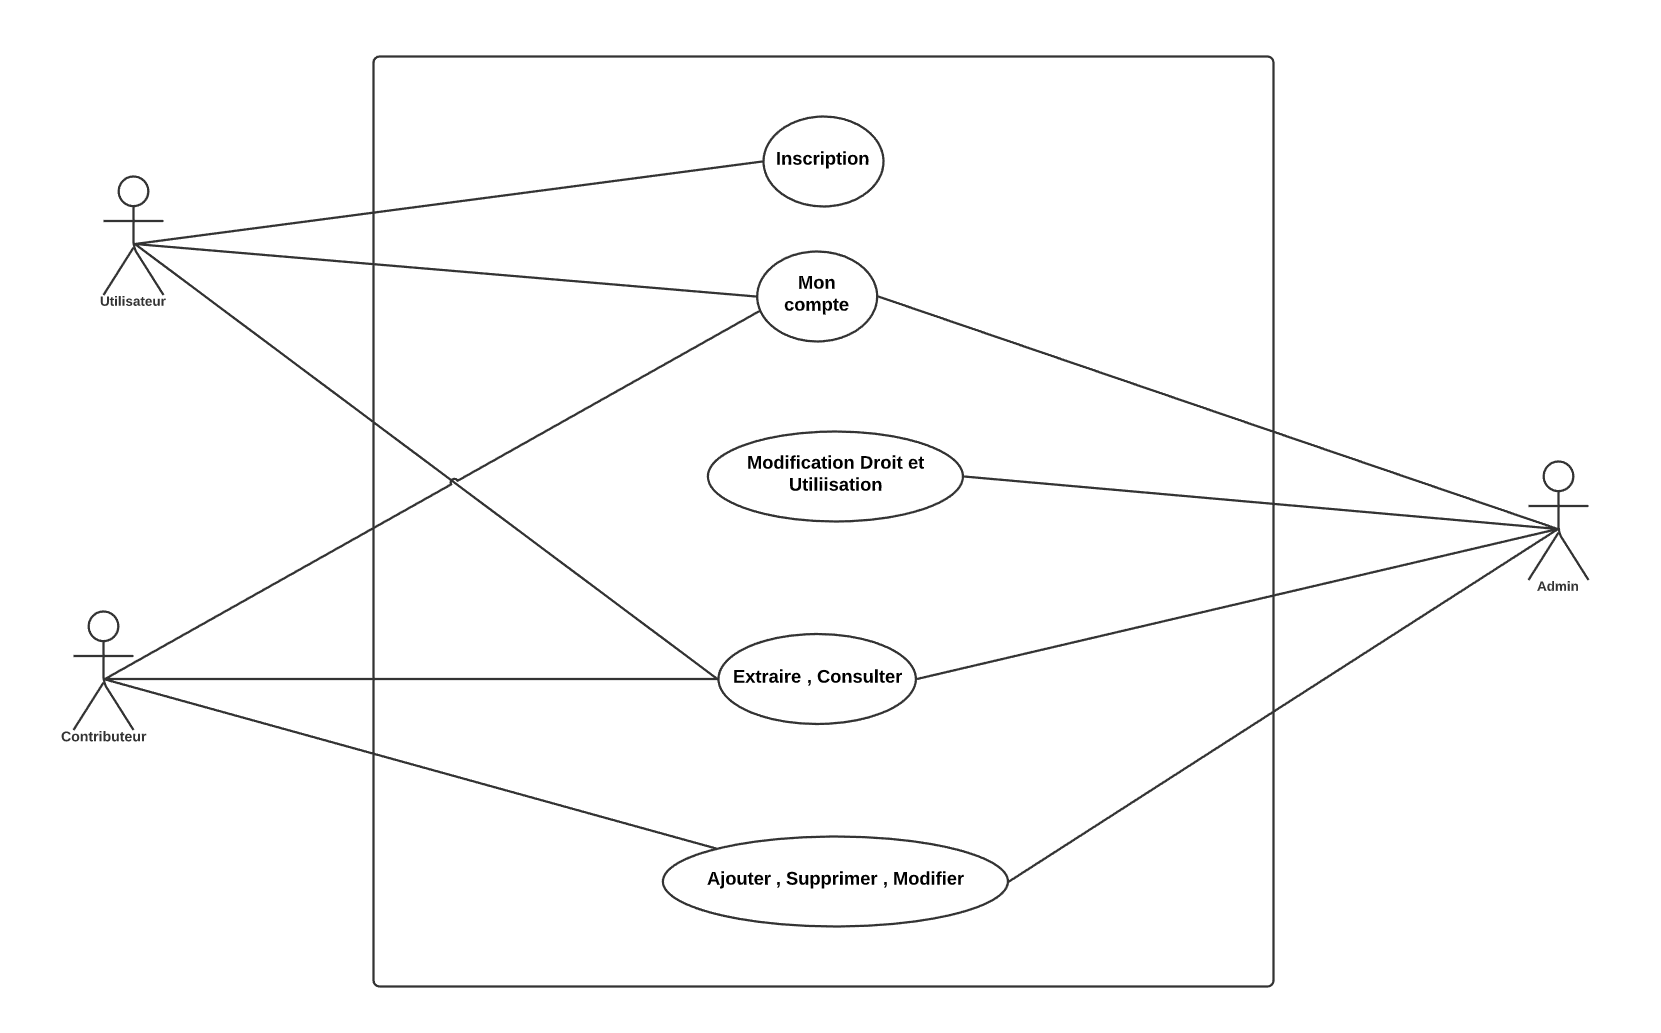
\includegraphics[scale=0.3]{uml.png}
    \caption{Gestion des rôles des utilisateurs }
\end{figure}


 \subsection{Exporter le LeFFF}

{Nous offrirons la possibilité d'exporter le \textbf{lexique} sélectionné avec un \textbf{filtre} afin que l'utilisateur puisse le \textbf{télécharger}\par}

\section{Les besoins non fonctionnels}

\subsection{Sécurité}
{Le système doit offrir un \textbf{accès personnalisé} pour nos utilisateurs (chacun à son rôle), de plus doit utiliser des \textbf{protocoles de sécurité} ou des certificats \textsc{Https} }

\subsection{Format de fichier}
Nous offrirons la possibilité de gérer le téléchargement du \textbf{LeFFF} ou d'une partie du \textbf{lexique} sous format \textbf{txt}.

\subsection{Performances}

{Nous devrons faire en sorte à ce que la \textbf{base de données} soit \textbf{optimisée} afin qu'une recherche ou exportation par de multiple personnes en même temps ne prenne par un temps trop grand.\par}
Nous sommes dans l'obligation de manipuler la \textbf{gestion de la mémoire} d'une manière très \textbf{efficace} dans le but d'assurer le fonctionnement des besoins fonctionnels dans tous les scénarios d'utilisation possible du logiciel. 

\subsection{Ergonomie}
L’ergonomie touche à la \textbf{qualité} et au \textbf{confort d’utilisation} de la navigation web, dans notre cas le client nous a donné une liberté dans le choix de l'agencement de la page, la police, les couleurs, le design. 
